\section{Meta-object system}
Meta-object system forms substantial part of Qt functionality, providing majority of Qt classes with ability to asynchronously report its state when something happens. Furthermore, you can equip even your custom classes with extra textual information, fetch names of your objects\index{object} at run time or make your classes use of the custom \textit{property system}\index{property system} that provides faster and syntactically unified access to your class member data.

\begin{fdocextra}
The word \enquote{meta} (which is originally Greek preposition, in Greek written as \enquote{\textmu \textepsilon \texttau \textalpha} was for the first time used by \textit{Aristotle}, the great Greek philosopher. Aristotle wrote plenty of writings, covering poetry, music or politics. His creations needed to be sorted later so that they could be interpreted correctly. Writings got sorted and scholars realized that there is one book with no name. It was placed \textit{after} Aristotle's great work \textit{Physics}. That's why that mysterious paper was named \textit{Metaphysics}, literally \enquote{the paper after Physics.}
\end{fdocextra}

\subsection{What is meta-object?}
Generally, meta-object is an entity that extends another object, providing us certain kind of information \textit{beyond} that particular object or set of objects. Meta-objects lie beyond actual objects, forming (kind of \enquote{higher}) abstraction layer of any Qt application. We can name this layer \textit{meta-echelon}\index{meta-echelon}.

Each class instance exposes its private data through \textit{methods} to its users -- other classes. Publicly available class members (methods or \textit{properties}\footnote{Property can be understood as private data member plus accessing getter/setter functions.}) form class interface, the only way to control class data and class behavior. This data is the only classical way to \enquote{see} the object from the view of its purpose but it says completely nothing about object inner structure and representation,\eg it doesn't expose type of on object (in run time) or count of its methods. Classic class methods do not provide us with \textit{meta-information}\index{meta-information}. Meta-objects do that.

\subsection{Reflection}
Ability to obtain and perhaps modify meta-information of any object is an action called \textit{introspection}\index{introspection} (or \textit{reflection})\index{reflection}. We can distinguish two kinds of reflection:
\begin{description}
\item[RUN TIME REFLECTION] \hfill \\
This is the superior way of reflection. Introspection of meta-information of certain object is possible at runtime but with one important addition. Compiler supporting run time reflection has absolutely no need to know the basis for meta-information construction at compile time. It does not need to add any extra data to the output code to allow reflection. Reflection is natural part of the language. This kind of reflection is supported primarily by languages that profit from using virtual machine\index{virtual machine} and special output executable file structure. Both Java and .NET-based languages (\eg \csharp or Visual Basic) provide this.
\item[COMPILE TIME REFLECTION] \hfill \\
Compiler of compile time reflection supported language has to do extra work to make reflection available. It usually produces extra code that grabs all (or most of) meta-information at compile time by going through the source code and extracting property names, method names, class names and other needed information. Extracted information is then formed into certain aggregations that are available as meta-objects at run time.

This approach makes the compilation little slower because an extra tool has to be executed to do the job. This concerns Qt. Qt uses meta-object compiler\index{meta-object compiler}\index{moc} to produce meta-objects.
\end{description}

\subsection{Qt meta-object system}
Qt uses compilation-based reflection due to \cpp language limitations. Each object created within Qt meta-object system is automatically equipped with shadow meta-object. This meta-object allows you to do amazing things with that particular object. You can obtain its class name, check if this object's class inherits another class, get name of the superclass or names of its methods. You can even call methods by their names stored in a string (\autoref{listing:invoke})! Complete example can be found in\fdocinlinecode{text}{!}{sources/laboratory/08-invoke} directory.

\begin{fdoccode}{cpp}{listing:invoke}{String-based method invokation in Qt meta-object system}
#include <QDebug>

#include <iostream>

#include "myapplication.h"


int main(int argc, char *argv[]){
    MyApplication a(argc, argv);
    
    std::string input;
    qDebug("Type name of method to be executed: ");
    std::cin >> input;
    QMetaObject::invokeMethod(&a, input.c_str());

    return a.exec();
}
\end{fdoccode}

\subsection{Enabling meta-object features for custom classes}
Not all classes in a Qt-based application take part in the meta-object system. You need to to several steps to make sure that objects of your class will be accompanied with corresponding meta-objects:

\begin{enumerate}
\item Your class needs to inherit\fdocinlinecode{cpp}{!}{QObject}. Public inheritance is recommended.\fdocinlinecode{cpp}{!}{QObject} class is fantastic base stone for any custom classes in Qt application. You will learn about it in the next chapter.
\item Your class needs to contain\fdocinlinecode{cpp}{!}{Q_OBJECT} macro in its private section, best way is right under class name. This macro adds several methods to your class, one of them is all important\fdocinlinecode{cpp}{!}{QMetaObject *metaObject() const} method. Moreover, dynamic translation system is enabled by this macro too. You will learn about Qt applications translation later.
\end{enumerate}

\subsection{QObject class -- the cradle of meta-objects}
\fdocinlinecode{cpp}{!}{QObject} class is the very base class for each meta-object-system-enabled class and provides many marvelous features. It is good to use\fdocinlinecode{cpp}{!}{QObject} as the base class even for your custom classes within any Qt application because there is one particularly amazing feature -- the automatic memory management provided by \nameref{section:model}.

\subsubsection{Qt object trees}\label{section:model}
There are some rules that apply to the way\fdocinlinecode{cpp}{!}{QObject} should be inherited. Copy constructor and assignment operator mustn't be implemented in inheriting class. Reasons are very simple:
\begin{enumerate}
\item Each and every\fdocinlinecode{cpp}{!}{QObject} instance stores pointer to its parent\fdocinlinecode{cpp}{!}{QObject} instance. This results in instance tree hierarchy (\autoref{figure:modeltree}). Should copy of\fdocinlinecode{cpp}{!}{QObject} instance point to the parent of the original\fdocinlinecode{cpp}{!}{QObject} instance?

Consider situation in the \autoref{figure:samenames}. \enquote{George} instance was cloned and placed in the hierarchy. In general, there is no rule on where to place new copy in the tree hierarchy. It could be positioned as the sibling of the original object. New \enquote{George} is the sibling of the original \enquote{George}. Problem becomes clear when the original \enquote{George} instance is freed from memory. All its children are removed too, in other words, whole subtree with \enquote{George} as the root gets cleared from application memory but another (cloned) \enquote{George} remains untouched. Is this desired behavior? In some situations it could be but sometimes it's not.

\item Each\fdocinlinecode{cpp}{!}{QObject} instance has certain properties and those can be unique. Example of such a property is instance name (can be set by\fdocinlinecode{cpp}{!}{void	QObject::setObjectName(const QString & name)} function) which should be unique for each\fdocinlinecode{cpp}{!}{QObject} instance. The same name could be automatically assigned to the new copy of the instance but that results in two instances with the same name (\autoref{figure:samenames}) and that's the problem because you may want to search for one particular object by name which is possible in Qt. Two objects with the same name make search ambiguous.
\end{enumerate}

\begin{figure}[ht]
\centering
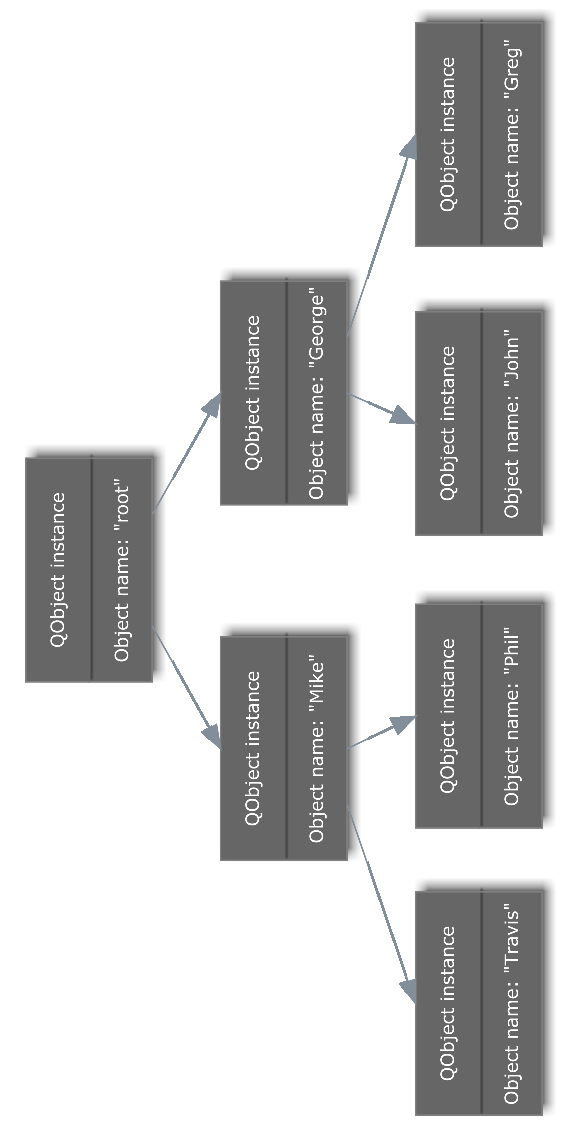
\includegraphics[angle=-90,width=13cm]{graphics/laboratory/12-modeltree.pdf}
\caption{QObject instances tree hierarchy}\label{figure:modeltree}
\end{figure}

\begin{figure}[ht]
\centering
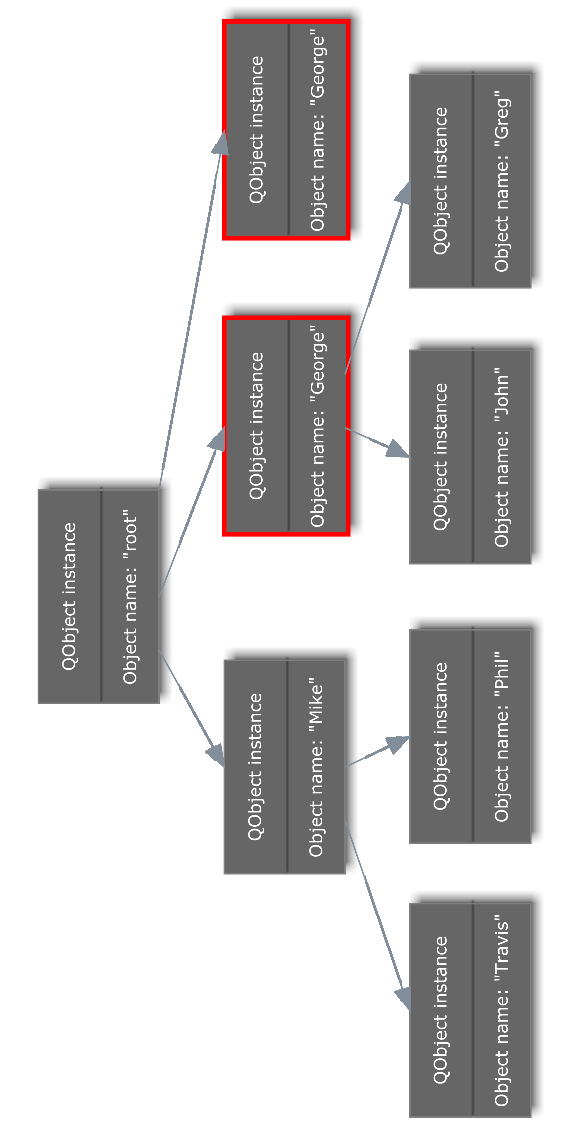
\includegraphics[angle=-90,width=13cm]{graphics/laboratory/13-samenames.pdf}
\caption{Broken QObject instances tree hierarchy}\label{figure:samenames}
\end{figure}

Every complex Qt-based application usually contains several\fdocinlinecode{cpp}{!}{QObject} tree hierarchies. These trees are disjunct. Example of typical tree hierarchy can be application main window. It usually contains menu bar, status bar, bunch of buttons, some text boxes and other visual elements. Naturally all these elements are owned by main windows. Thus, main window is the root of the main window elements tree hierarchy. If main windows is cleared from memory, then all its children are cleared from memory too which is desired behavior. This behavior makes memory management more automatic.

\indent\fdocinlinecode{cpp}{!}{QObject}-based object can be deleted from memory by calling\fdocinlinecode{cpp}{!}{this->deleteLater()} method or by using classic\fdocinlinecode{cpp}{!}{delete} operator. See more about deleting objects in Qt in \autoref{section:events}.

Existence of tree hierarchies impacts positively on several topics:
\begin{itemize}
\item more sophisticated memory management\footnote{Tree hierarchies form just part of Qt memory management as you will see in \autoref{section:memorym}.}
\item better track of the number of objects in application component
\item better debugging
\end{itemize}

\subsubsection{Subclassing QObject}
You have already read something about\fdocinlinecode{cpp}{!}{QObject} class in previous paragraphs. You know that\fdocinlinecode{cpp}{!}{QObject} instances form tree hierarchy. Subclassing\fdocinlinecode{cpp}{!}{QObject} is similar to standard \cpp class subclassing but you need to include\fdocinlinecode{cpp}{!}{Q_OBJECT} macro and you should instantiate\fdocinlinecode{cpp}{!}{QObject} with correct parent object, except some rare cases. Inheriting\fdocinlinecode{cpp}{!}{QObject} is very simple, just see \autoref{listing:qobjecti}.

You see that\fdocinlinecode{cpp}{!}{QObject} constructor accepts pointer to parent object which is used to construct\fdocinlinecode{cpp}{!}{QObject} base for\fdocinlinecode{cpp}{!}{MyQObject} instances.

\begin{fdoccode}{cpp}{listing:qobjecti}{Subclassing QObject}
/* header file (myqobject.h) */
class MyQObject : public QObject {
	Q_OBJECT
	
    public:
		explicit MyQObject(QObject *parent = 0);
};

/* source file (myqobject.cpp) */
#include "myqobject.h"


MyQObject::MyQObject(QObject *parent) : QObject(parent) {
}
\end{fdoccode}
%% případně ještě dynamic cast a QPointer a custom type.

\subsubsection{Signal--slot mechanism}
Signal--slot mechanism is the main tool to interconnect two \fdocinlinecode{cpp}{!}{QObject}-based objects, allowing thread-safe communication between them. Signals and slots form alternative to the callback mechanism. 

\begin{description}\label{desc:sig}
\item[What is signal?] \hfill \\
Signal is sign, which signs occurrence of specific event that happened during method execution of particular\fdocinlinecode{cpp}{!}{QObject}-based class. In fact, specially formed method.
\item[What is slot?] \hfill \\
Slot is method in the same or another class which represents natural reaction to the signal occurrence.
\end{description}

\begin{figure}[ht]
\centering

\includegraphics[width=8cm]{graphics/laboratory/14-ss-textbox.png}
\caption{Typical textbox example}\label{figure:ss-textbox}
\end{figure}

Imagine typical \textit{textbox}\index{textbox} control (\autoref{figure:ss-textbox}). This textbox could offers many \textit{signals} which are usual for this kind of control. Every textbox should emit appropriate signal if its content changes or if ENTER key is pressed by application user.

So there is textbox which emits signals. We need to have receiver of signals too. Receiver of signals from textbox could be for example the application. Application can perform some action (for example exit) if ENTER key is pressed inside textbox. Such an action is called \textit{slot}. If there exists slot in one particular entity that reacts to signals emitted by another entity, then we say that there is \textit{signal--slot connection} between these two entities.

One signal (of one entity) can be connected to several slots (contained in several entities), this behavior represents 1\text{:}N relationship. Several signals can be connected to one slot (M\text{:}1 relationship). Existence of 1\text{:}1 relationship is obvious.

Signal--slot mechanism does not applies just to \fdocabbrevref{GUI} elements. Every\fdocinlinecode{cpp}{!}{QObject} subclass can take advantage of it. Simple example can be file downloader class which signals progress of download.

\begin{fdocextra}
Tiny definitions of signal and slot on page \pageref{desc:sig} correspond with terms \index{event} and \index{delegate} known from .NET-based languages. \citep[p.~200-202]{nigel:csharp}
\end{fdocextra}

\paragraph{Using signal--slot mechanism}
We are familiar with basic terms now. We are also able to subclass QObject. Let's implement very simple bank account representation. We expect that account provides us with possibility to save/withdraw money, check its status or make payments to another account.

Accounts are usually managed by bank. Bank ensures us that our payments are sent to correct target accounts. Sample application can be found in\fdocinlinecode{text}{!}{sources/laboratory/11-bank} subdirectory. Let's dig into the application.

Application contains two primary classes:\fdocinlinecode{cpp}{!}{Account} and\fdocinlinecode{cpp}{!}{Bank}. Let's start with\fdocinlinecode{cpp}{!}{Account} class (see \autoref{listing:acc-head}). This class inherits\fdocinlinecode{cpp}{!}{QObject} (lines \ref{listing:qobj1}-\ref{listing:qobj2}), thus, meta-object features (including signal--slot mechanism) are available. Slots declaration is preceded by\fdocinlinecode{cpp}{!}{slots} keyword (line \ref{listing:slots1}) with any modifier. You can have public slot as well as private slot. It's just a matter of situation. As stated earlier, slot is just method with special rights.

\begin{fdoccode}{cpp}{listing:acc-head}{Account class design}
class Account : public QObject {(*@\label{listing:qobj1}@*)
	Q_OBJECT(*@\label{listing:qobj2}@*)

    public:
		explicit Account(const QString &owner,
						int deposit,
						Bank *parent);

		// These are NOT slots.
		void status();
		QString name();

    public slots:(*@\label{listing:slots1}@*)
		// Used by customer who requests money from his account.
		// Customer can be either bank or account owner.
		void withdrawMoney(int sum);

		// Used by customer to save money to this account.
		// Customer can be either bank or account owner.
		void saveMoney(int sum);(*@\label{listing:slots2}@*)

    signals:
		// Emitted when money is withdrawn successfully from this account.
		void withdrawn(int sum);

		// Emitted when money is saved successfully into this account.
		void saved(int sum);

    private:
		QString m_owner;
		int m_deposit;
};
\end{fdoccode}

\subsubsection{QObject instance life cycle}
% Q_OBJECT, QObject, object model, metaobject compiler, property system